% Options for packages loaded elsewhere
\PassOptionsToPackage{unicode}{hyperref}
\PassOptionsToPackage{hyphens}{url}
%
\documentclass[
]{article}
\usepackage{amsmath,amssymb}
\usepackage{iftex}
\ifPDFTeX
  \usepackage[T1]{fontenc}
  \usepackage[utf8]{inputenc}
  \usepackage{textcomp} % provide euro and other symbols
\else % if luatex or xetex
  \usepackage{unicode-math} % this also loads fontspec
  \defaultfontfeatures{Scale=MatchLowercase}
  \defaultfontfeatures[\rmfamily]{Ligatures=TeX,Scale=1}
\fi
\usepackage{lmodern}
\ifPDFTeX\else
  % xetex/luatex font selection
\fi
% Use upquote if available, for straight quotes in verbatim environments
\IfFileExists{upquote.sty}{\usepackage{upquote}}{}
\IfFileExists{microtype.sty}{% use microtype if available
  \usepackage[]{microtype}
  \UseMicrotypeSet[protrusion]{basicmath} % disable protrusion for tt fonts
}{}
\makeatletter
\@ifundefined{KOMAClassName}{% if non-KOMA class
  \IfFileExists{parskip.sty}{%
    \usepackage{parskip}
  }{% else
    \setlength{\parindent}{0pt}
    \setlength{\parskip}{6pt plus 2pt minus 1pt}}
}{% if KOMA class
  \KOMAoptions{parskip=half}}
\makeatother
\usepackage{xcolor}
\usepackage[margin=1in]{geometry}
\usepackage{longtable,booktabs,array}
\usepackage{calc} % for calculating minipage widths
% Correct order of tables after \paragraph or \subparagraph
\usepackage{etoolbox}
\makeatletter
\patchcmd\longtable{\par}{\if@noskipsec\mbox{}\fi\par}{}{}
\makeatother
% Allow footnotes in longtable head/foot
\IfFileExists{footnotehyper.sty}{\usepackage{footnotehyper}}{\usepackage{footnote}}
\makesavenoteenv{longtable}
\usepackage{graphicx}
\makeatletter
\def\maxwidth{\ifdim\Gin@nat@width>\linewidth\linewidth\else\Gin@nat@width\fi}
\def\maxheight{\ifdim\Gin@nat@height>\textheight\textheight\else\Gin@nat@height\fi}
\makeatother
% Scale images if necessary, so that they will not overflow the page
% margins by default, and it is still possible to overwrite the defaults
% using explicit options in \includegraphics[width, height, ...]{}
\setkeys{Gin}{width=\maxwidth,height=\maxheight,keepaspectratio}
% Set default figure placement to htbp
\makeatletter
\def\fps@figure{htbp}
\makeatother
\setlength{\emergencystretch}{3em} % prevent overfull lines
\providecommand{\tightlist}{%
  \setlength{\itemsep}{0pt}\setlength{\parskip}{0pt}}
\setcounter{secnumdepth}{5}
   \usepackage{xcolor}
   \usepackage{threeparttablex}
   \usepackage{longtable}
   \usepackage{subfig}
   \usepackage{mathptmx}
   \usepackage{unicode-math}
%\setmainfont{Latin Modern Roman} 
%\setmathfont{STIXTwoMath-Regular}
   \usepackage[scaled=1.1]{helvet}
   \renewcommand{\familydefault}{\rmdefault}
   

\newcommand{\bibfont}{\footnotesize}

%   \usepackage[authordate, backend=bibtex,sorting=nyt, natbib, ]{biblatex-chicago}
%   \usepackage[authordate]{biblatex-chicago}
%\DeclareFieldFormat[article]{title}{\mkbibquote{#1}} % make article titles in quotes
% \DeclareFieldFormat[thesis]{title}{\mkbibemph{#1}} % make theses italics

   \renewcommand{\bibfont}{\small}
   \usepackage{babel}
   \usepackage{fancyhdr}
   \usepackage{setspace}
   \usepackage{caption}
   \pagestyle{fancy}
   \usepackage{siunitx}
   \usepackage[capposition=top]{floatrow}
   \usepackage{dsfont}
   \usepackage{placeins}
   \usepackage{todonotes}
\usepackage[subfigure]{tocloft}
\usepackage{pgffor}
   \usepackage{csquotes}
   \usepackage[toc,page,title,titletoc,header]{appendix}    
   \usepackage{amsthm} % to introduce theorems etc.
   \usepackage{bm}
   \usepackage{bbm}  % Define \bm{} to use bold math fonts
   \usepackage{amssymb}
   \newtheorem{Theorem}{Theorem}
   \newtheorem{fact}{Fact}
   \newtheorem{mydef}{Definition}
   \usepackage[hang]{footmisc}	% Footnote formatting
   \renewcommand{\hangfootparindent}{1em}
   \renewcommand{\hangfootparskip}{0em}
   \renewcommand{\footnotemargin}{0.00001pt}
   \def\footnotelayout{\hspace{1em}}%
   \def\footnotelayout{\hspace{1em}}%
   \renewcommand\thepart{\hspace{1cm} \arabic{part}}
   \renewcommand\thesection{\Roman{section}}
   \renewcommand\thesubsection{\thesection.\arabic{subsection}}
   \renewcommand\thesubsubsection{\Alph{subsubsection}}
   \renewcommand\theparagraph{\alph{paragraph})}
   \renewcommand\thesubparagraph{\roman{subparagraph})}
   \usepackage[nobottomtitles*]{titlesec}
   \titleformat{\chapter}[display]{\normalfont\huge\bfseries}{\chaptertitlename\ \thechapter.}{20pt}{\Huge}
   \titleformat{\section}{\normalfont\Large\bfseries}{\thesection}{1em}{}
   \titleformat{\subsection}{\normalfont\large\bfseries}{\thesubsection}{1em}{}
   \titleformat{\subsubsection}{\normalfont\normalsize\bfseries}{\thesubsubsection)}{1em}{}
   \titleformat{\paragraph}[runin]{\normalfont\normalsize\bfseries}{\theparagraph}{1em}{}
   \titleformat{\subparagraph}[runin]{\normalfont\normalsize\bfseries}{\thesubparagraph}{1em}{}
   \titlespacing*{\chapter} {0pt}{50pt}{40pt}
   \titlespacing*{\section} {12pt}{3.5ex plus 1ex minus .2ex}{2.3ex plus .2ex}
   \titlespacing*{\subsection} {24pt}{3.25ex plus 1ex minus .2ex}{1.5ex plus .2ex}
   \titlespacing*{\subsubsection}{36pt}{3.25ex plus 1ex minus .2ex}{1.5ex plus .2ex}
   \titlespacing*{\paragraph} {0pt}{3.25ex plus 1ex minus .2ex}{1em}
   \titlespacing*{\subparagraph} {24pt}{3.25ex plus 1ex minus .2ex}{1em}
   

   
   \newcommand{\esp}[1]{\mathds{E}[ #1 ]}
   \newcommand{\espb}[1]{\mathds{E}\Big[ #1 \Big]}
   \newcommand{\var}[1]{\mathds{V}[ #1 ]}
   \newcommand{\one}[1]{\mathds{1}( #1 )}
   \newcommand{\normal}[1]{\mathcal{N}}
   \usepackage{etoolbox} %— available from CTAN (required)–
   \usepackage{keyval}%— a standard package (required)–
   \usepackage{ifthen}%— a standard package (required)–
   \usepackage{graphicx} % You need this for the headers
   \definecolor{ForestGreen}{RGB}{34,139,34}
   \usepackage{booktabs}
    \newcolumntype{d}{S[
      input-open-uncertainty=,
      input-close-uncertainty=,
      parse-numbers = false,
      table-align-text-pre=false,
      table-align-text-post=false
       ]}
    \usepackage{algorithm}
    %\usepackage{algorithm2e}
    \usepackage{algpseudocode}
     \usepackage{pgfgantt}
     \usepackage{tikz}
     \usetikzlibrary{arrows.meta}
      \usetikzlibrary{arrows}
      \usetikzlibrary{patterns}
      \usepackage{fontspec}
      \setmainfont{Times New Roman}
      \renewcommand\qedsymbol{\emph{QED}}
      \newcommand\blfootnote[1]{%
      \begingroup
      \renewcommand\thefootnote{}\footnote{#1}%
      \addtocounter{footnote}{-1}%
      \endgroup}
      
% add more space for table and figure to avoid floating
\renewcommand{\topfraction}{.85}
\renewcommand{\bottomfraction}{.7}
\renewcommand{\textfraction}{.15}
\renewcommand{\floatpagefraction}{.66}
\setcounter{topnumber}{3}
\setcounter{bottomnumber}{3}
\setcounter{totalnumber}{4}

%\AtBeginDocument{\let\maketitle\relax}      
\usepackage{flafter}
\usepackage{float}
\usepackage{tabularray}
\usepackage[normalem]{ulem}
\usepackage{graphicx}
\UseTblrLibrary{booktabs}
\UseTblrLibrary{rotating}
\UseTblrLibrary{siunitx}
\NewTableCommand{\tinytableDefineColor}[3]{\definecolor{#1}{#2}{#3}}
\newcommand{\tinytableTabularrayUnderline}[1]{\underline{#1}}
\newcommand{\tinytableTabularrayStrikeout}[1]{\sout{#1}}
\usepackage{fontspec}
\usepackage{multirow}
\usepackage{multicol}
\usepackage{colortbl}
\usepackage{hhline}
\newlength\Oldarrayrulewidth
\newlength\Oldtabcolsep
\usepackage{longtable}
\usepackage{array}
\usepackage{hyperref}
\usepackage{wrapfig}
\ifLuaTeX
  \usepackage{selnolig}  % disable illegal ligatures
\fi
\usepackage[]{natbib}
\bibliographystyle{plainnat}
\usepackage{bookmark}
\IfFileExists{xurl.sty}{\usepackage{xurl}}{} % add URL line breaks if available
\urlstyle{same}
\hypersetup{
  pdftitle={Investigating how administrative burden and search costs affect social inequalities in early childcare access},
  pdfauthor={Arthur Heim},
  hidelinks,
  pdfcreator={LaTeX via pandoc}}

\title{Investigating how administrative burden and search costs affect social inequalities in early childcare access}
\usepackage{etoolbox}
\makeatletter
\providecommand{\subtitle}[1]{% add subtitle to \maketitle
  \apptocmd{\@title}{\par {\large #1 \par}}{}{}
}
\makeatother
\subtitle{Draft of a formal model}
\author{Arthur Heim}
\date{2025-01-31}

\usepackage{amsthm}
\newtheorem{theorem}{Theorem}[section]
\newtheorem{lemma}{Lemma}[section]
\newtheorem{corollary}{Corollary}[section]
\newtheorem{proposition}{Proposition}[section]
\newtheorem{conjecture}{Conjecture}[section]
\theoremstyle{definition}
\newtheorem{definition}{Definition}[section]
\theoremstyle{definition}
\newtheorem{example}{Example}[section]
\theoremstyle{definition}
\newtheorem{exercise}{Exercise}[section]
\theoremstyle{definition}
\newtheorem{hypothesis}{Hypothesis}[section]
\theoremstyle{remark}
\newtheorem*{remark}{Remark}
\newtheorem*{solution}{Solution}
\begin{document}
\maketitle

\section{Setting}\label{setting}

We model the decision to apply for childcare as a function of perceived eligibility, transaction costs, and potential benefits. Households face uncertainty regarding their eligibility and the costs associated with the application process. The intervention aims to reduce these frictions through information provision and administrative support.

We define latent variables with a superscript \(V^*\) and a measurement of that varriable as \(V\).

We consider a sequential decision process where at the first period (baseline),
a pregnant woman has \emph{ex-ante} unobserved \textbf{preference profile} \(\theta^*_0\) with regard to future childcare options. We observe a set of attributes \(\mathbf{X}\) and intention to use \(I_0\). Among \(\mathbf{X}\), there are social group metrics (\(G\)) such as SES status (based on education), migration background, and rough metrics of temporal preferences \(\rho\) and knowledge of childcare \(\mathcal{I}\), which capture latent traits \(\rho^*\) and \(\mathcal{I}^*\) with error. There are also cognitive and structural factor that may hinder decisions. Let \(\mathcal{C}\) denote the subjective application costs.
Without loss of generality, let \(\mathbf{Z}\) denote the set of observable \(\mathbf{X}\) supplemented with random shocks such as treatments.

\subsection{Intention gap by social groups}\label{intention-gap-by-social-groups}

Formally, the gap between two sets of values of covariates \(\mathbf{x}\) \(\mathbf{x^\prime}\) in intention to use at baseline is:

\begin{equation}
\Delta_{x,x'}(I_{0}) = \espb{I_{0i}|\mathbf{X}=\mathbf{x}}-\espb{I_{0i}|\mathbf{X}=\mathbf{x^\prime}}
\end{equation}

With a random sample, these conditional differences in reported intention to use childcare can be estimated using OLS and heteroskedasticity robust standard errors (Linear probability model) or by first estimating a model with parametric restrictions on \(I_0^*\) (such as logit or probit) and computing marginal effects.

However, these parameters and sample analogues are only descriptive difference in means between two groups who also differs in observable characteristics and latent \(U_I\).

\subsection{Application and access gap in the endline data}\label{application-and-access-gap-in-the-endline-data}

The endline survey includes the different sets of outcomes including some metrics of knowledges, application behaviours and access to formal childcare. We leave attrition issues for now and focus on application behaviours. We come back to these points later.

Let \(\tilde{Y_i}=\one{\text{applied to any childcare}}\) be the endline measure of application behaviours which derive from:
\[
\tilde{Y}_{i}=\underbrace{\one{\text{applied for childminders}}}_{Y^c}+\underbrace{\one{\text{applied for daycare}}}_{Y^d}\\
\]
In practice, \(\tilde{Y}\) also include other childcare arrangement.

The application gap is :

\begin{equation}
\Delta_{x,x'}(\tilde{Y}_i) = \espb{\tilde{Y}_i|\mathbf{X}=\mathbf{x}}-\espb{\tilde{Y}_i|\mathbf{X}=\mathbf{x^\prime}}
\end{equation}

Denoting \(\tilde{Y^*}\) the variable for access to formal childcare, The access gap is :

\begin{equation}
\Delta_{x,x'}(\tilde{Y*}_i) = \espb{\tilde{Y^*}_i|\mathbf{X}=\mathbf{x}}-\espb{\tilde{Y^*}_i|\mathbf{X}=\mathbf{x^\prime}}
\end{equation}

In our setting, the covariates are discrete. These three parameters can therefore be estimated from the control group by regressing the outcome on group dummies using OLS and heterokedasticity robust standard errors, or by computing marginal effects from a logit or probit model.

In practice, we simply estimate:
\begin{equation}
W_i = \alpha_w +\beta_w X+ \upsilon_{iw}
\end{equation}
Where \(W_i\) denotes any outcome and \(X\) one of the social group or subjective attribute variable we test.

Results are are reported in Figure \ref{fig:AttentionAction}.

\begin{figure}[H]
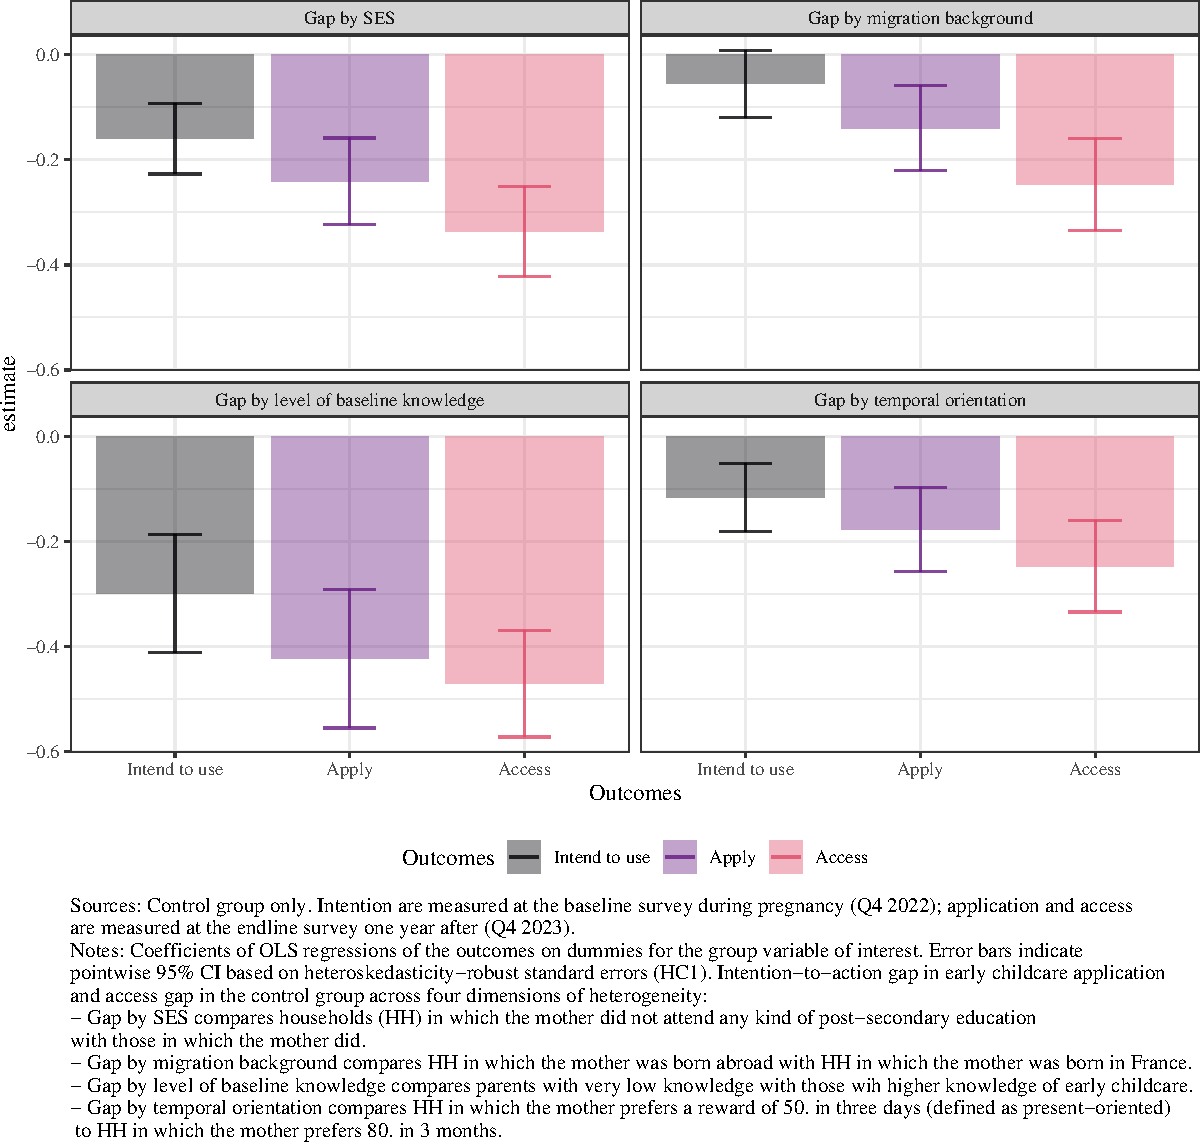
\includegraphics[width=1\linewidth]{Theory_files/figure-latex/AttentionAction-1} \caption{ The intention-to-action gap in early childcare application and access in the control group across four dimensions of heterogeneity. Intention to use early childcare is measured at the baseline survey during pregnancy. Early childcare application and early childcare access are measured at the endline survey one year after.}\label{fig:AttentionAction}
\end{figure}

\begin{figure}
\centering
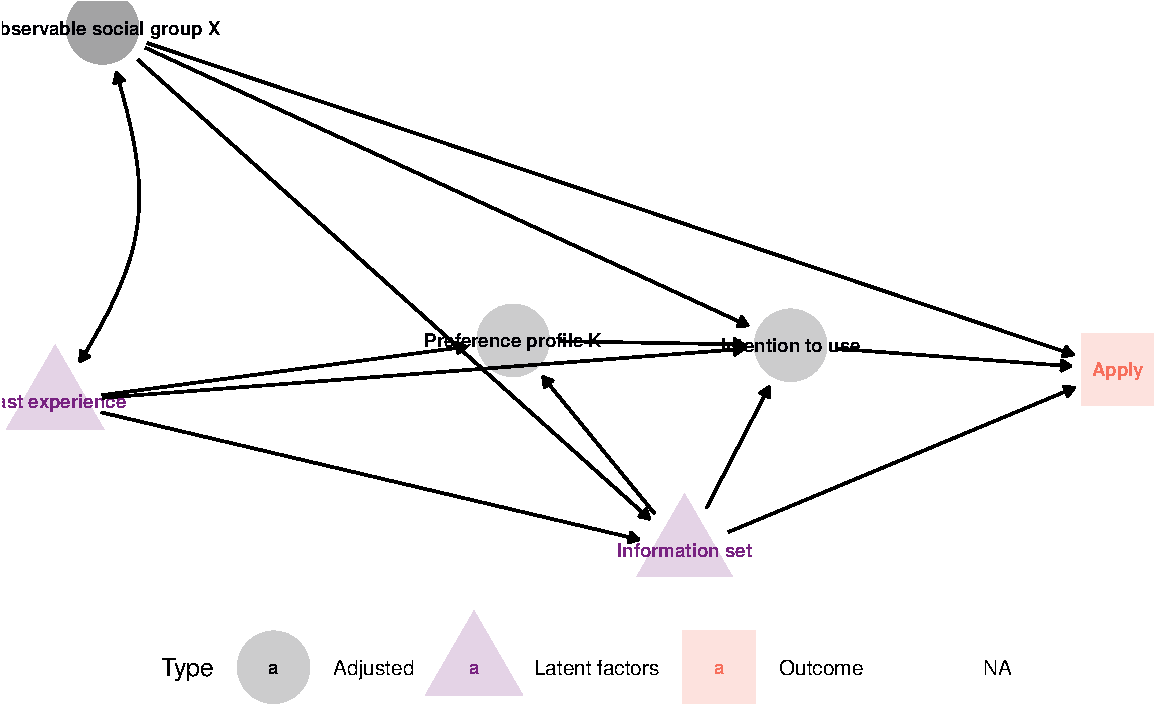
\includegraphics{Theory_files/figure-latex/DagIntention-1.pdf}
\caption{\label{fig:DagIntention}How observed baseline characteristics relate with the main outcome.}
\end{figure}

\subsection{Intention to action gap}\label{intention-to-action-gap}

Another parameter of interest is the average intention to action gap \(i.e.\) the expected individual difference \(\esp{Y_i-I_{0i}}\) , and differences between social groups. to be clear, this variable equals 0 when people are consistent in their reported intention and application behaviours, equals 1 when the person applied but did'nt intend to (\emph{Switchers}) and -1 when they intended to but did not apply (\emph{Quitters}).

\[
\begin{aligned}
\esp{Y_i-I_{0i}}=&Pr(Y_i>I_{0i})\underbrace{\esp{Y_i-I_{0i}>0}}_{=1}+Pr(Y_i=I_{0i})\underbrace{\esp{Y_i-I_{0i}=0}}_{=0}+Pr(Y_i<I_{0i})\underbrace{\esp{Y_i-I_{0i}<0}}_{=-1}\\
=&\underbrace{Pr(Y_i>I_{0i})}_{switchers}-\underbrace{Pr(Y_i<I_{0i})}_{quitters}
\end{aligned}
\]

\begin{proof}
Starting with \(\mathbb{E}[Y_i - I_{0i}]\), we can decompose this expectation by considering all possible cases for the difference \(Y_i - I_{0i}\) and using the law of iterated expectation.

Since \(Y_i\) and \(I_{0i}\) are binary (0 or 1):

\begin{itemize}
\tightlist
\item
  When \(Y_i > I_{0i}\), we must have \(Y_i = 1\) and \(I_{0i} = 0\), so \(Y_i - I_{0i} = 1\)
\item
  When \(Y_i = I_{0i}\), we have \(Y_i - I_{0i} = 0\)
\item
  When \(Y_i < I_{0i}\), we must have \(Y_i = 0\) and \(I_{0i} = 1\), so \(Y_i - I_{0i} = -1\)
\end{itemize}

Therefore:

\begin{itemize}
\tightlist
\item
  \(\mathbb{E}[Y_i - I_{0i} | Y_i > I_{0i}] = 1\)
\item
  \(\mathbb{E}[Y_i - I_{0i} | Y_i = I_{0i}] = 0\)
\item
  \(\mathbb{E}[Y_i - I_{0i} | Y_i < I_{0i}] = -1\)
\end{itemize}

Using the law of iterated expectation:
\[
\begin{aligned}
\esp{Y_i - I_{0i}} = &\Pr(Y_i > I_{0i}) \cdot \mathbb{E}[Y_i - I_{0i} | Y_i > I_{0i}] + \Pr(Y_i = I_{0i}) \cdot \mathbb{E}[Y_i - I_{0i} | Y_i = I_{0i}] \\
 &+ \Pr(Y_i < I{0i}) \cdot \mathbb{E}[Y_i - I_{0i} | Y_i < I_{0i}]
\end{aligned}
\]
Continuing with the derivation:
\[
\mathbb{E}[Y_i - I_{0i}] = \Pr(Y_i > I_{0i}) \cdot 1 + \Pr(Y_i = I_{0i}) \cdot 0 + \Pr(Y_i < I_{0i}) \cdot (-1)
\]
The term \(\Pr(Y_i = I_{0i}) \cdot 0\) drops out, and we're left with:
\[
\mathbb{E}[Y_i - I_{0i}] = \Pr(Y_i > I_{0i}) - \Pr(Y_i < I_{0i})
\]
\end{proof}

\ref{fig:figQuitters} below estimate these three quantities in the control group:

\begin{figure}
\centering
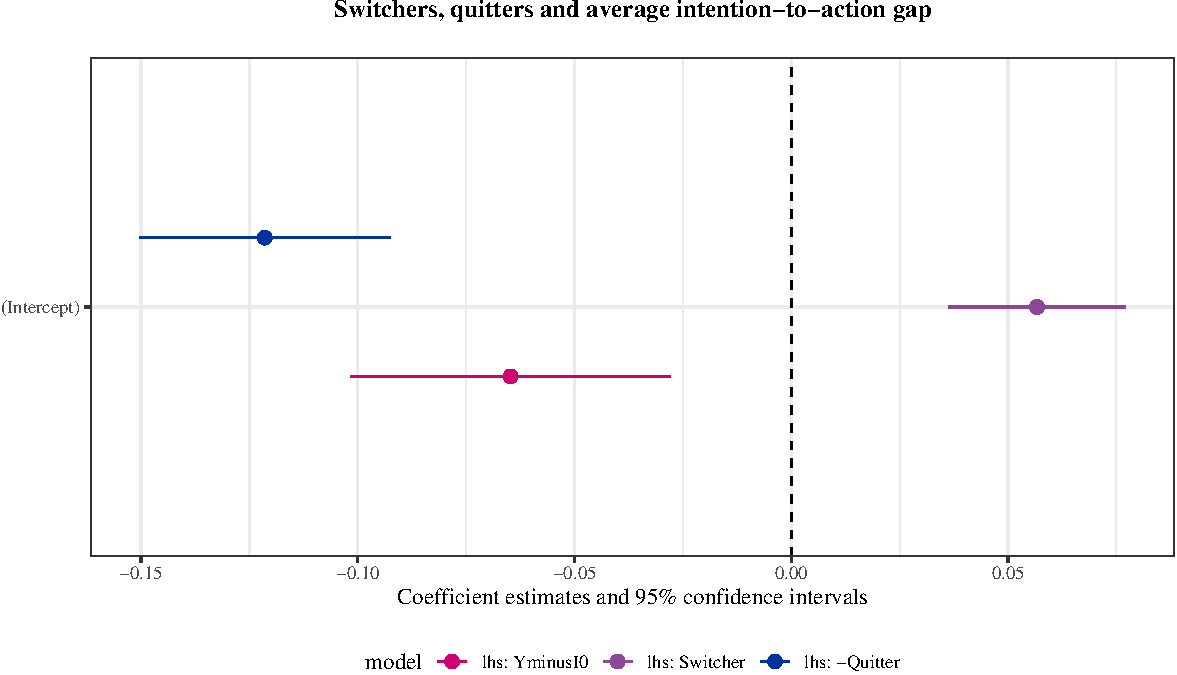
\includegraphics{Theory_files/figure-latex/figQuitters-1.pdf}
\caption{\label{fig:figQuitters}Intention to action gap: switchers and quitters}
\end{figure}

The intention-to-action gap is -6.5\% ; it sums the 5.7\% of \emph{switchers} (who did not intend but applied) and the -12.1\% of \emph{quitters}.

We can go further into the decomposition using the same expansion.
The probability of being a switcher can be divided into the probability of for high and low SES weighted by their relative share in the sample:

For each SES group, we can write:
\[
\begin{aligned}
\Pr(Y_{i} > I_{0i} | SES_i = High) =& \Pr(Y_i = 1, I_{0i} = 0 | SES_i = High)&\\
\Pr(Y_{i} > I_{0i} | SES_i = Low ) =& \Pr(Y_i = 1, I_{0i} = 0 | SES_i = Low)&
\end{aligned}
\]
These conditional probabilities can be further decomposed using Bayes' rule:
\[
\begin{aligned}
\Pr(Y_i = 1, I{0i} = 0 | SES_i = High)& = \Pr(Y_i = 1 | I_{0i} = 0, SES_i = High) \times \Pr(I_{0i} = 0 | SES_i = High)\\
\Pr(Y_i = 1, I{0i} = 0 | SES_i = Low )& = \Pr(Y_i = 1 | I_{0i} = 0, SES_i = Low ) \times \Pr(I_{0i} = 0 | SES_i = Low)
\end{aligned}
\]
Putting it all together, we get:
\[
\begin{aligned}
\Pr(Y_i > I0) =& \left[\Pr(Y_i = 1 | I_{0i} = 0, SEi = High) \times \Pr(I_{0i} = 0 | SES_i = High) \times Pr(SES_i = High)\right] +\\
&\left[\Pr(Y_i = 1 | I_{0i} = 0, SES_i = Low) \times \Pr(I_{0i} = 0 | SES_i = Low) \times Pr(SES_i = Low)\right]
\end{aligned}
\]
This decomposition allows us to quantify:

The contribution of the High SES group to the overall switching probability:
\begin{equation}
\Pr(Y_i > I_{0i}, SES_i = High) = \Pr(Y_i = 1 | I_{0i} = 0, SES_i = High) \times \Pr(I_{0i} = 0 | SES_i = High) \times \Pr(SES_i = High)
\end{equation}
The contribution of the Low SES group to the overall switching probability:
\begin{equation}
Pr(Y > I0, SES = Low) = Pr(Y = 1 | I0 = 0, SES = Low) \times Pr(I0 = 0 | SES = Low) \times Pr(SES = Low)
\end{equation}

This decomposition gives hiw much of the overall switching behaviour is driven by each SES group, accounting for both their population share and their propensity to switch. We can do the same derivation for quitters.

We end-up here with a decomposition of the intention-to-action gap as a weighted average of the switching and quitting share in high and low SES group with weights proportional to the share of household who did not intend to use daycare in each group times the share of each group in the sample.

\begin{figure}
\centering
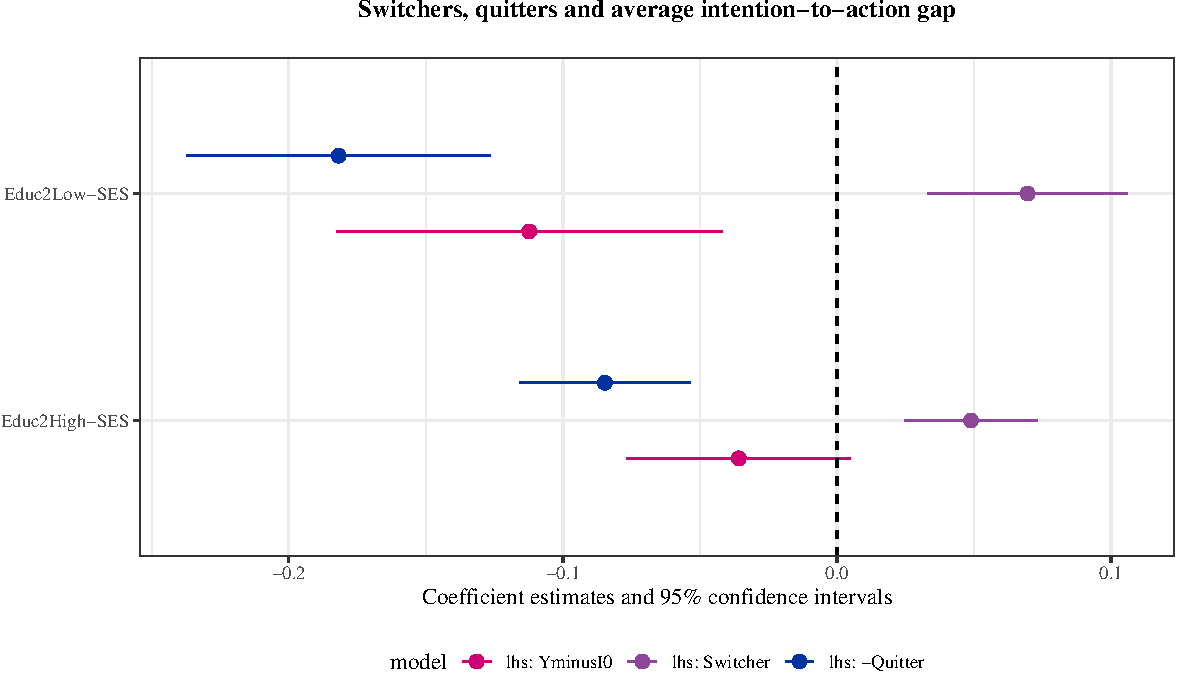
\includegraphics{Theory_files/figure-latex/figQuittersECS-1.pdf}
\caption{\label{fig:figQuittersECS}Intention to action gap: switchers and quitters}
\end{figure}

These results show that for High SES, the intention-to-action gap (I.A.G) is small and not significant with that sample size. It is significant for Low-SES group and we later test if the two are different. The I.A.G of High-SES group averages 5\% of switchers and the -8\%n of quitters.

The I.A.G of Low-SES group averages 7\% of switchers and the -18\%n of quitters.

\begin{figure}
\centering
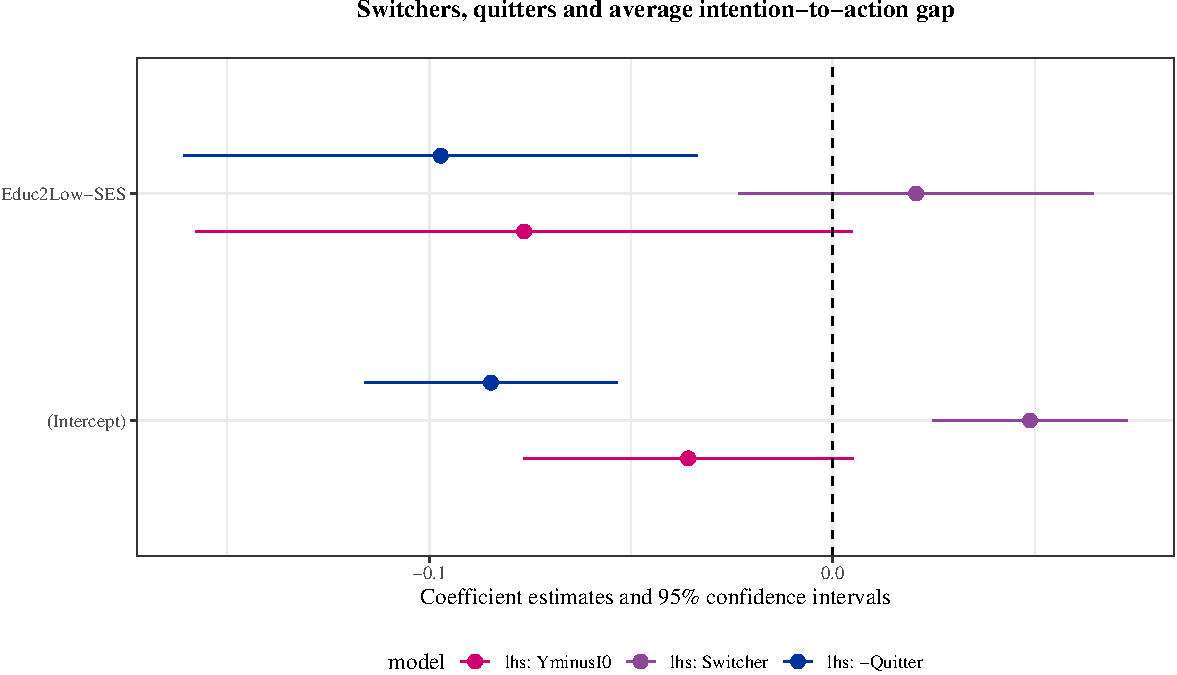
\includegraphics{Theory_files/figure-latex/figQuitterslin-1.pdf}
\caption{\label{fig:figQuitterslin}Intention to action gap: switchers and quitters by SES}
\end{figure}

\begin{table}
\centering
\begin{talltblr}[         %% tabularray outer open
caption={Intention to action gap by SES: tests},
note{}={* p \num{< 0.1}, ** p \num{< 0.05}, *** p \num{< 0.01}},
]                     %% tabularray outer close
{                     %% tabularray inner open
colspec={Q[]Q[]Q[]Q[]},
column{2,3,4}={}{halign=c,},
column{1}={}{halign=l,},
hline{6}={1,2,3,4}{solid, black, 0.05em},
}                     %% tabularray inner close
\toprule
& lhs: YminusI0 & lhs: Switcher & lhs: -Quitter \\ \midrule %% TinyTableHeader
(Intercept) & \num{-0.036}* & \num{0.049}*** & \num{-0.085}*** \\
& (\num{0.021}) & (\num{0.012}) & (\num{0.016}) \\
Educ2Low-SES & \num{-0.076}* & \num{0.021} & \num{-0.097}*** \\
& (\num{0.041}) & (\num{0.022}) & (\num{0.032}) \\
Num.Obs. & \num{494} & \num{494} & \num{494} \\
R2 & \num{0.008} & \num{0.002} & \num{0.021} \\
R2 Adj. & \num{0.006} & \num{-0.000} & \num{0.019} \\
Std.Errors & Heteroskedasticity-robust & Heteroskedasticity-robust & Heteroskedasticity-robust \\
\bottomrule
\end{talltblr}
\end{table}

Note that there is a direct link between the intention gap and application gap by social group defined earlier:

\[
\begin{aligned}
\Delta_{x,x'}(\tilde{Y}_i) -\Delta_{x,x'}(I_{0})&=& \espb{\tilde{Y}_i|\mathbf{X}=\mathbf{x}}-\espb{\tilde{Y}_i|\mathbf{X}=\mathbf{x^\prime}}-(\espb{I_{0i}|\mathbf{X}=\mathbf{x}}-\espb{I_{0i}|\mathbf{X}=\mathbf{x^\prime}})\\
 &=&\espb{\tilde{Y}_i-I_{0i}|\mathbf{X}=\mathbf{x}}-\espb{\tilde{Y}_i-I_{0i}|\mathbf{X}=\mathbf{x^\prime}}
 \end{aligned}
\]

\begin{align}
\Delta_{x,x'}(\tilde{Y}_i-I_{0i}) &=& \espb{\tilde{Y}_i-I_{0i}|\mathbf{X}=\mathbf{x}}-\espb{\tilde{Y}_i-I_{0i}|\mathbf{X}=\mathbf{x^\prime}}%\\
%&=&  \underbrace{\espb{\tilde{Y}_i|\mathbf{X}=\mathbf{x}}-\espb{\tilde{Y}_i|\mathbf{X}=\mathbf{x^\prime}}}_{\Delta_{x,x'}(\tilde{Y}_i)}-\underbrace{\left(\espb{I_{0i}|\mathbf{X}=\mathbf{x}}-\espb{I_{0i}|\mathbf{X}=\mathbf{x^\prime}}\right)}_{\Delta_{x,x'}(I_{0i})}
\end{align}

Thus, these parameters can be estimated either by regressing the difference between application and intention on social group dummies or by:

\begin{enumerate}
\def\labelenumi{\arabic{enumi})}
\tightlist
\item
  stacking baseline (intention) and endline databases (application)
\item
  defining an outcome \(Y\) which equals \(I_0\) in the baseline and \(\tilde{Y}\) in the endline.
\item
  regressing Y on an endline dummy, an interaction with the group indicator, mother fixed effects and clustered SE
\end{enumerate}

The coefficient of the interaction is an estimate of \(\Delta_{x,x'}(\tilde{Y}_i-I_{0i})\) i.e.~the intention-to-action gap between high and low SES.

\begin{table}
\centering
\begin{talltblr}[         %% tabularray outer open
caption={Intention to application gap by SES status},
note{}={* p \num{< 0.1}, ** p \num{< 0.05}, *** p \num{< 0.01}},
]                     %% tabularray outer close
{                     %% tabularray inner open
colspec={Q[]Q[]Q[]Q[]Q[]},
column{2,3,4,5}={}{halign=c,},
column{1}={}{halign=l,},
hline{12}={1,2,3,4,5}{solid, black, 0.05em},
}                     %% tabularray inner close
\toprule
& Mean gap & Group average & OLS & DID \\ \midrule %% TinyTableHeader
(Intercept) & \num{-0.065}*** &  & \num{-0.036}* &  \\
& (\num{0.019}) &  & (\num{0.021}) &  \\
Educ2High-SES &  & \num{-0.036}* &  &  \\
&  & (\num{0.021}) &  &  \\
Educ2Low-SES &  & \num{-0.112}*** & \num{-0.076}* &  \\
&  & (\num{0.036}) & (\num{0.041}) &  \\
Baseline &  &  &  & \num{-0.036}* \\
&  &  &  & (\num{0.021}) \\
Baseline × Educ2Low-SES &  &  &  & \num{-0.076}* \\
&  &  &  & (\num{0.041}) \\
Num.Obs. & \num{494} & \num{494} & \num{494} & \num{1117} \\
R2 &  & \num{0.006} & \num{0.008} & \num{0.781} \\
R2 Adj. &  & \num{0.004} & \num{0.006} & \num{0.503} \\
Std.Errors & Heteroskedasticity-robust & Heteroskedasticity-robust & Heteroskedasticity-robust & by: ResponseId \\
FE: ResponseId &  &  &  & X \\
\bottomrule
\end{talltblr}
\end{table}

Table \ref{tab:IntendToAction} shows these estimates by high/low education. The average individual gap among high SES is -3.6pp, which average switchers from intention to no use and from no intention to use among high SES households. It decomposes the total intention to action gap. This gap is wider for Low SES Family ; the difference in intention to action gap between the two groups is driven by the second and third columns, both estimating the difference in difference in gaps, either by using the actual difference in variable as outcome, or stacking databases with interactions.

In Table \ref{tab:IntendToAction2}, we test the difference in the share of quitters and switchers by social groups. For switchers, there are no difference by SES status But for quitters, Low-SES status who are already less likely to intend to use childcare are twice more likely to quit !

\begin{table}
\centering
\begin{talltblr}[         %% tabularray outer open
caption={Intention to application gap by SES status},
note{}={* p \num{< 0.1}, ** p \num{< 0.05}, *** p \num{< 0.01}},
]                     %% tabularray outer close
{                     %% tabularray inner open
colspec={Q[]Q[]Q[]Q[]Q[]},
column{2,3,4,5}={}{halign=c,},
column{1}={}{halign=l,},
hline{8}={1,2,3,4,5}{solid, black, 0.05em},
}                     %% tabularray inner close
\toprule
& Group lhs: Switcher & Group lhs: -Quitter & Diff lhs: Switcher & Diff lhs: -Quitter \\ \midrule %% TinyTableHeader
Educ2High-SES & \num{0.049}*** & \num{-0.085}*** &  &  \\
& (\num{0.012}) & (\num{0.016}) &  &  \\
Educ2Low-SES & \num{0.070}*** & \num{-0.182}*** & \num{0.021} & \num{-0.097}*** \\
& (\num{0.019}) & (\num{0.028}) & (\num{0.022}) & (\num{0.032}) \\
(Intercept) &  &  & \num{0.049}*** & \num{-0.085}*** \\
&  &  & (\num{0.012}) & (\num{0.016}) \\
Num.Obs. & \num{494} & \num{494} & \num{494} & \num{494} \\
R2 & \num{-0.000} & \num{0.019} & \num{0.002} & \num{0.021} \\
R2 Adj. & \num{-0.002} & \num{0.017} & \num{-0.000} & \num{0.019} \\
\bottomrule
\end{talltblr}
\end{table}

\section{Treatment effects on quitter and switchers.}\label{treatment-effects-on-quitter-and-switchers.}

Now that we have seen that there are more quitters than switchers and that the gap in quitters is twice as large among low SES group, we look at the effect of information and administrative support on these probabilities.

\subsection{Average estimations}\label{average-estimations}

\global\setlength{\Oldarrayrulewidth}{\arrayrulewidth}

\global\setlength{\Oldtabcolsep}{\tabcolsep}

\setlength{\tabcolsep}{2pt}

\renewcommand*{\arraystretch}{1.5}



\providecommand{\ascline}[3]{\noalign{\global\arrayrulewidth #1}\arrayrulecolor[HTML]{#2}\cline{#3}}

\begin{longtable}[c]{|p{0.94in}|p{1.06in}|p{1.06in}}

\caption{ITT\ on\ Switching\ and\ quitting\ status}\label{tab:unnamed-chunk-2}\\

\ascline{1.5pt}{666666}{1-3}

\multicolumn{1}{>{\centering}m{\dimexpr 0.94in+0\tabcolsep}}{\textcolor[HTML]{000000}{\fontsize{11}{11}\selectfont{\global\setmainfont{Times New Roman}{\ }}}} & \multicolumn{1}{>{\centering}m{\dimexpr 1.06in+0\tabcolsep}}{\textcolor[HTML]{000000}{\fontsize{11}{11}\selectfont{\global\setmainfont{Times New Roman}{Quitter}}}} & \multicolumn{1}{>{\centering}m{\dimexpr 1.06in+0\tabcolsep}}{\textcolor[HTML]{000000}{\fontsize{11}{11}\selectfont{\global\setmainfont{Times New Roman}{Switchers}}}} \\

\ascline{1.5pt}{666666}{1-3}\endfirsthead \caption[]{ITT\ on\ Switching\ and\ quitting\ status}\label{tab:unnamed-chunk-2}\\

\ascline{1.5pt}{666666}{1-3}

\multicolumn{1}{>{\centering}m{\dimexpr 0.94in+0\tabcolsep}}{\textcolor[HTML]{000000}{\fontsize{11}{11}\selectfont{\global\setmainfont{Times New Roman}{\ }}}} & \multicolumn{1}{>{\centering}m{\dimexpr 1.06in+0\tabcolsep}}{\textcolor[HTML]{000000}{\fontsize{11}{11}\selectfont{\global\setmainfont{Times New Roman}{Quitter}}}} & \multicolumn{1}{>{\centering}m{\dimexpr 1.06in+0\tabcolsep}}{\textcolor[HTML]{000000}{\fontsize{11}{11}\selectfont{\global\setmainfont{Times New Roman}{Switchers}}}} \\

\ascline{1.5pt}{666666}{1-3}\endhead



\multicolumn{3}{>{\raggedright}m{\dimexpr 3.07in+4\tabcolsep}}{\textcolor[HTML]{000000}{\fontsize{11}{11}\selectfont{\global\setmainfont{Times New Roman}{Sources:\ stacked\ database\ of\ pairwise\ comparisons.\ }}}\textcolor[HTML]{000000}{\fontsize{11}{11}\selectfont{\global\setmainfont{Times New Roman}{\linebreak }}}\textcolor[HTML]{000000}{\fontsize{11}{11}\selectfont{\global\setmainfont{Times New Roman}{\ \ \ \ \ \ *=\ p<.1,\ **=\ p<.05,\ ***=\ p<.01\ based\ on\ point-wise\ p-value.}}}\textcolor[HTML]{000000}{\fontsize{11}{11}\selectfont{\global\setmainfont{Times New Roman}{\linebreak }}}\textcolor[HTML]{000000}{\fontsize{11}{11}\selectfont{\global\setmainfont{Times New Roman}{\ \ \ \ \ \ Standard\ errors\ are\ cluster-heteroskedasticity\ robust\ adjusted\ at\ the\ block\ x\ wave\ level.}}}\textcolor[HTML]{000000}{\fontsize{11}{11}\selectfont{\global\setmainfont{Times New Roman}{\linebreak }}}\textcolor[HTML]{000000}{\fontsize{11}{11}\selectfont{\global\setmainfont{Times New Roman}{\ \ \ \ \ \ Adjusted\ p-value\ and\ confidence\ intervals\ account\ for\ simultaneous\ inference\ using\ the\ Westfall\ method.\ }}}\textcolor[HTML]{000000}{\fontsize{11}{11}\selectfont{\global\setmainfont{Times New Roman}{\linebreak }}}\textcolor[HTML]{000000}{\fontsize{11}{11}\selectfont{\global\setmainfont{Times New Roman}{\ \ \ \ \ \ Each\ column\ estimates\ jointly\ the\ effects\ of\ the\ program\ using\ fully-saturated\ stacked\ regressions.\ Control\ means\ estimated\ separately\ by\ OLS.}}}\textcolor[HTML]{000000}{\fontsize{11}{11}\selectfont{\global\setmainfont{Times New Roman}{\linebreak }}}\textcolor[HTML]{000000}{\fontsize{11}{11}\selectfont{\global\setmainfont{Times New Roman}{\ \ \ \ \ \ Joint\ significance\ test\ of\ null\ effect\ using\ Chi-2\ test\ and\ p-value\ are\ reported\ at\ the\ bottom\ of\ the\ table.}}}} \\

\endlastfoot



\multicolumn{1}{>{\centering}m{\dimexpr 0.94in+0\tabcolsep}}{\textcolor[HTML]{000000}{\fontsize{11}{11}\selectfont{\global\setmainfont{Times New Roman}{Information-only\ vs\ Control\ }}}} & \multicolumn{1}{>{\centering}m{\dimexpr 1.06in+0\tabcolsep}}{\textcolor[HTML]{000000}{\fontsize{11}{11}\selectfont{\global\setmainfont{Times New Roman}{-0.00\ (0.02)}}}} & \multicolumn{1}{>{\centering}m{\dimexpr 1.06in+0\tabcolsep}}{\textcolor[HTML]{000000}{\fontsize{11}{11}\selectfont{\global\setmainfont{Times New Roman}{-0.01\ (0.01)}}}} \\





\multicolumn{1}{>{\centering}m{\dimexpr 0.94in+0\tabcolsep}}{\textcolor[HTML]{000000}{\fontsize{11}{11}\selectfont{\global\setmainfont{Times New Roman}{}}}} & \multicolumn{1}{>{\centering}m{\dimexpr 1.06in+0\tabcolsep}}{\textcolor[HTML]{000000}{\fontsize{11}{11}\selectfont{\global\setmainfont{Times New Roman}{[-0.05,\ 0.04]}}}} & \multicolumn{1}{>{\centering}m{\dimexpr 1.06in+0\tabcolsep}}{\textcolor[HTML]{000000}{\fontsize{11}{11}\selectfont{\global\setmainfont{Times New Roman}{[-0.03,\ 0.01]}}}} \\





\multicolumn{1}{>{\centering}m{\dimexpr 0.94in+0\tabcolsep}}{\textcolor[HTML]{000000}{\fontsize{11}{11}\selectfont{\global\setmainfont{Times New Roman}{}}}} & \multicolumn{1}{>{\centering}m{\dimexpr 1.06in+0\tabcolsep}}{\textcolor[HTML]{000000}{\fontsize{11}{11}\selectfont{\global\setmainfont{Times New Roman}{adj.p.val.\ =\ 0.829}}}} & \multicolumn{1}{>{\centering}m{\dimexpr 1.06in+0\tabcolsep}}{\textcolor[HTML]{000000}{\fontsize{11}{11}\selectfont{\global\setmainfont{Times New Roman}{adj.p.val.\ =\ 0.553}}}} \\





\multicolumn{1}{>{\centering}m{\dimexpr 0.94in+0\tabcolsep}}{\textcolor[HTML]{000000}{\fontsize{11}{11}\selectfont{\global\setmainfont{Times New Roman}{Information\ +\ Support\ vs\ Control}}}} & \multicolumn{1}{>{\centering}m{\dimexpr 1.06in+0\tabcolsep}}{\textcolor[HTML]{000000}{\fontsize{11}{11}\selectfont{\global\setmainfont{Times New Roman}{-0.04**\ (0.02)}}}} & \multicolumn{1}{>{\centering}m{\dimexpr 1.06in+0\tabcolsep}}{\textcolor[HTML]{000000}{\fontsize{11}{11}\selectfont{\global\setmainfont{Times New Roman}{0.00\ (0.01)}}}} \\





\multicolumn{1}{>{\centering}m{\dimexpr 0.94in+0\tabcolsep}}{\textcolor[HTML]{000000}{\fontsize{11}{11}\selectfont{\global\setmainfont{Times New Roman}{}}}} & \multicolumn{1}{>{\centering}m{\dimexpr 1.06in+0\tabcolsep}}{\textcolor[HTML]{000000}{\fontsize{11}{11}\selectfont{\global\setmainfont{Times New Roman}{[-0.08,\ 0.00]}}}} & \multicolumn{1}{>{\centering}m{\dimexpr 1.06in+0\tabcolsep}}{\textcolor[HTML]{000000}{\fontsize{11}{11}\selectfont{\global\setmainfont{Times New Roman}{[-0.03,\ 0.03]}}}} \\





\multicolumn{1}{>{\centering}m{\dimexpr 0.94in+0\tabcolsep}}{\textcolor[HTML]{000000}{\fontsize{11}{11}\selectfont{\global\setmainfont{Times New Roman}{}}}} & \multicolumn{1}{>{\centering}m{\dimexpr 1.06in+0\tabcolsep}}{\textcolor[HTML]{000000}{\fontsize{11}{11}\selectfont{\global\setmainfont{Times New Roman}{adj.p.val.\ =\ 0.060}}}} & \multicolumn{1}{>{\centering}m{\dimexpr 1.06in+0\tabcolsep}}{\textcolor[HTML]{000000}{\fontsize{11}{11}\selectfont{\global\setmainfont{Times New Roman}{adj.p.val.\ =\ 0.719}}}} \\





\multicolumn{1}{>{\centering}m{\dimexpr 0.94in+0\tabcolsep}}{\textcolor[HTML]{000000}{\fontsize{11}{11}\selectfont{\global\setmainfont{Times New Roman}{Information\ +\ support\ vs\ Information-only}}}} & \multicolumn{1}{>{\centering}m{\dimexpr 1.06in+0\tabcolsep}}{\textcolor[HTML]{000000}{\fontsize{11}{11}\selectfont{\global\setmainfont{Times New Roman}{-0.04*\ (0.02)}}}} & \multicolumn{1}{>{\centering}m{\dimexpr 1.06in+0\tabcolsep}}{\textcolor[HTML]{000000}{\fontsize{11}{11}\selectfont{\global\setmainfont{Times New Roman}{0.01\ (0.01)}}}} \\





\multicolumn{1}{>{\centering}m{\dimexpr 0.94in+0\tabcolsep}}{\textcolor[HTML]{000000}{\fontsize{11}{11}\selectfont{\global\setmainfont{Times New Roman}{}}}} & \multicolumn{1}{>{\centering}m{\dimexpr 1.06in+0\tabcolsep}}{\textcolor[HTML]{000000}{\fontsize{11}{11}\selectfont{\global\setmainfont{Times New Roman}{[-0.08,\ 0.01]}}}} & \multicolumn{1}{>{\centering}m{\dimexpr 1.06in+0\tabcolsep}}{\textcolor[HTML]{000000}{\fontsize{11}{11}\selectfont{\global\setmainfont{Times New Roman}{[-0.02,\ 0.04]}}}} \\





\multicolumn{1}{>{\centering}m{\dimexpr 0.94in+0\tabcolsep}}{\textcolor[HTML]{000000}{\fontsize{11}{11}\selectfont{\global\setmainfont{Times New Roman}{}}}} & \multicolumn{1}{>{\centering}m{\dimexpr 1.06in+0\tabcolsep}}{\textcolor[HTML]{000000}{\fontsize{11}{11}\selectfont{\global\setmainfont{Times New Roman}{adj.p.val.\ =\ 0.094}}}} & \multicolumn{1}{>{\centering}m{\dimexpr 1.06in+0\tabcolsep}}{\textcolor[HTML]{000000}{\fontsize{11}{11}\selectfont{\global\setmainfont{Times New Roman}{adj.p.val.\ =\ 0.672}}}} \\

\ascline{1pt}{666666}{1-3}



\multicolumn{1}{>{\centering}m{\dimexpr 0.94in+0\tabcolsep}}{\textcolor[HTML]{000000}{\fontsize{11}{11}\selectfont{\global\setmainfont{Times New Roman}{Mean\ control\ group}}}} & \multicolumn{1}{>{\centering}m{\dimexpr 1.06in+0\tabcolsep}}{\textcolor[HTML]{000000}{\fontsize{11}{11}\selectfont{\global\setmainfont{Times New Roman}{0.12\ (0.02)}}}} & \multicolumn{1}{>{\centering}m{\dimexpr 1.06in+0\tabcolsep}}{\textcolor[HTML]{000000}{\fontsize{11}{11}\selectfont{\global\setmainfont{Times New Roman}{0.05\ (0.01)}}}} \\





\multicolumn{1}{>{\centering}m{\dimexpr 0.94in+0\tabcolsep}}{\textcolor[HTML]{000000}{\fontsize{11}{11}\selectfont{\global\setmainfont{Times New Roman}{}}}} & \multicolumn{1}{>{\centering}m{\dimexpr 1.06in+0\tabcolsep}}{\textcolor[HTML]{000000}{\fontsize{11}{11}\selectfont{\global\setmainfont{Times New Roman}{[0.08,\ 0.16]}}}} & \multicolumn{1}{>{\centering}m{\dimexpr 1.06in+0\tabcolsep}}{\textcolor[HTML]{000000}{\fontsize{11}{11}\selectfont{\global\setmainfont{Times New Roman}{[0.02,\ 0.09]}}}} \\

\ascline{1pt}{666666}{1-3}



\multicolumn{1}{>{\centering}m{\dimexpr 0.94in+0\tabcolsep}}{\textcolor[HTML]{000000}{\fontsize{11}{11}\selectfont{\global\setmainfont{Times New Roman}{Num.Obs.}}}} & \multicolumn{1}{>{\centering}m{\dimexpr 1.06in+0\tabcolsep}}{\textcolor[HTML]{000000}{\fontsize{11}{11}\selectfont{\global\setmainfont{Times New Roman}{2906}}}} & \multicolumn{1}{>{\centering}m{\dimexpr 1.06in+0\tabcolsep}}{\textcolor[HTML]{000000}{\fontsize{11}{11}\selectfont{\global\setmainfont{Times New Roman}{2906}}}} \\





\multicolumn{1}{>{\centering}m{\dimexpr 0.94in+0\tabcolsep}}{\textcolor[HTML]{000000}{\fontsize{11}{11}\selectfont{\global\setmainfont{Times New Roman}{R2}}}} & \multicolumn{1}{>{\centering}m{\dimexpr 1.06in+0\tabcolsep}}{\textcolor[HTML]{000000}{\fontsize{11}{11}\selectfont{\global\setmainfont{Times New Roman}{0.144}}}} & \multicolumn{1}{>{\centering}m{\dimexpr 1.06in+0\tabcolsep}}{\textcolor[HTML]{000000}{\fontsize{11}{11}\selectfont{\global\setmainfont{Times New Roman}{0.354}}}} \\





\multicolumn{1}{>{\centering}m{\dimexpr 0.94in+0\tabcolsep}}{\textcolor[HTML]{000000}{\fontsize{11}{11}\selectfont{\global\setmainfont{Times New Roman}{R2\ Adj.}}}} & \multicolumn{1}{>{\centering}m{\dimexpr 1.06in+0\tabcolsep}}{\textcolor[HTML]{000000}{\fontsize{11}{11}\selectfont{\global\setmainfont{Times New Roman}{0.062}}}} & \multicolumn{1}{>{\centering}m{\dimexpr 1.06in+0\tabcolsep}}{\textcolor[HTML]{000000}{\fontsize{11}{11}\selectfont{\global\setmainfont{Times New Roman}{0.292}}}} \\





\multicolumn{1}{>{\centering}m{\dimexpr 0.94in+0\tabcolsep}}{\textcolor[HTML]{000000}{\fontsize{11}{11}\selectfont{\global\setmainfont{Times New Roman}{Fixed\ effects}}}} & \multicolumn{1}{>{\centering}m{\dimexpr 1.06in+0\tabcolsep}}{\textcolor[HTML]{000000}{\fontsize{11}{11}\selectfont{\global\setmainfont{Times New Roman}{X}}}} & \multicolumn{1}{>{\centering}m{\dimexpr 1.06in+0\tabcolsep}}{\textcolor[HTML]{000000}{\fontsize{11}{11}\selectfont{\global\setmainfont{Times New Roman}{X}}}} \\





\multicolumn{1}{>{\centering}m{\dimexpr 0.94in+0\tabcolsep}}{\textcolor[HTML]{000000}{\fontsize{11}{11}\selectfont{\global\setmainfont{Times New Roman}{Chi\ 2}}}} & \multicolumn{1}{>{\centering}m{\dimexpr 1.06in+0\tabcolsep}}{\textcolor[HTML]{000000}{\fontsize{11}{11}\selectfont{\global\setmainfont{Times New Roman}{6.43}}}} & \multicolumn{1}{>{\centering}m{\dimexpr 1.06in+0\tabcolsep}}{\textcolor[HTML]{000000}{\fontsize{11}{11}\selectfont{\global\setmainfont{Times New Roman}{4.45}}}} \\





\multicolumn{1}{>{\centering}m{\dimexpr 0.94in+0\tabcolsep}}{\textcolor[HTML]{000000}{\fontsize{11}{11}\selectfont{\global\setmainfont{Times New Roman}{P-value}}}} & \multicolumn{1}{>{\centering}m{\dimexpr 1.06in+0\tabcolsep}}{\textcolor[HTML]{000000}{\fontsize{11}{11}\selectfont{\global\setmainfont{Times New Roman}{0.092}}}} & \multicolumn{1}{>{\centering}m{\dimexpr 1.06in+0\tabcolsep}}{\textcolor[HTML]{000000}{\fontsize{11}{11}\selectfont{\global\setmainfont{Times New Roman}{0.217}}}} \\

\ascline{1.5pt}{666666}{1-3}



\end{longtable}



\arrayrulecolor[HTML]{000000}

\global\setlength{\arrayrulewidth}{\Oldarrayrulewidth}

\global\setlength{\tabcolsep}{\Oldtabcolsep}

\renewcommand*{\arraystretch}{1}

\subsection{Analysis by SES Status:}\label{analysis-by-ses-status}

\global\setlength{\Oldarrayrulewidth}{\arrayrulewidth}

\global\setlength{\Oldtabcolsep}{\tabcolsep}

\setlength{\tabcolsep}{2pt}

\renewcommand*{\arraystretch}{1.5}



\providecommand{\ascline}[3]{\noalign{\global\arrayrulewidth #1}\arrayrulecolor[HTML]{#2}\cline{#3}}

\begin{longtable}[c]{|p{0.94in}|p{0.94in}|p{1.06in}|p{1.06in}}



\ascline{1.5pt}{666666}{1-4}

\multicolumn{1}{>{\centering}m{\dimexpr 0.94in+0\tabcolsep}}{\textcolor[HTML]{000000}{\fontsize{11}{11}\selectfont{\global\setmainfont{Times New Roman}{Group}}}} & \multicolumn{1}{>{\centering}m{\dimexpr 0.94in+0\tabcolsep}}{\textcolor[HTML]{000000}{\fontsize{11}{11}\selectfont{\global\setmainfont{Times New Roman}{\ }}}} & \multicolumn{1}{>{\centering}m{\dimexpr 1.06in+0\tabcolsep}}{\textcolor[HTML]{000000}{\fontsize{11}{11}\selectfont{\global\setmainfont{Times New Roman}{Quitters}}}} & \multicolumn{1}{>{\centering}m{\dimexpr 1.06in+0\tabcolsep}}{\textcolor[HTML]{000000}{\fontsize{11}{11}\selectfont{\global\setmainfont{Times New Roman}{Switchers}}}} \\

\ascline{1.5pt}{666666}{1-4}\endfirsthead 

\ascline{1.5pt}{666666}{1-4}

\multicolumn{1}{>{\centering}m{\dimexpr 0.94in+0\tabcolsep}}{\textcolor[HTML]{000000}{\fontsize{11}{11}\selectfont{\global\setmainfont{Times New Roman}{Group}}}} & \multicolumn{1}{>{\centering}m{\dimexpr 0.94in+0\tabcolsep}}{\textcolor[HTML]{000000}{\fontsize{11}{11}\selectfont{\global\setmainfont{Times New Roman}{\ }}}} & \multicolumn{1}{>{\centering}m{\dimexpr 1.06in+0\tabcolsep}}{\textcolor[HTML]{000000}{\fontsize{11}{11}\selectfont{\global\setmainfont{Times New Roman}{Quitters}}}} & \multicolumn{1}{>{\centering}m{\dimexpr 1.06in+0\tabcolsep}}{\textcolor[HTML]{000000}{\fontsize{11}{11}\selectfont{\global\setmainfont{Times New Roman}{Switchers}}}} \\

\ascline{1.5pt}{666666}{1-4}\endhead



\multicolumn{1}{>{\centering}m{\dimexpr 0.94in+0\tabcolsep}}{\textcolor[HTML]{000000}{\fontsize{11}{11}\selectfont{\global\setmainfont{Times New Roman}{High-SES}}}} & \multicolumn{1}{>{\centering}m{\dimexpr 0.94in+0\tabcolsep}}{\textcolor[HTML]{000000}{\fontsize{11}{11}\selectfont{\global\setmainfont{Times New Roman}{Information-only\ vs\ Control\ }}}} & \multicolumn{1}{>{\centering}m{\dimexpr 1.06in+0\tabcolsep}}{\textcolor[HTML]{000000}{\fontsize{11}{11}\selectfont{\global\setmainfont{Times New Roman}{0.01\ (0.02)}}}} & \multicolumn{1}{>{\centering}m{\dimexpr 1.06in+0\tabcolsep}}{\textcolor[HTML]{000000}{\fontsize{11}{11}\selectfont{\global\setmainfont{Times New Roman}{-0.01\ (0.01)}}}} \\





\multicolumn{1}{>{\centering}m{\dimexpr 0.94in+0\tabcolsep}}{\textcolor[HTML]{000000}{\fontsize{11}{11}\selectfont{\global\setmainfont{Times New Roman}{}}}} & \multicolumn{1}{>{\centering}m{\dimexpr 0.94in+0\tabcolsep}}{\textcolor[HTML]{000000}{\fontsize{11}{11}\selectfont{\global\setmainfont{Times New Roman}{}}}} & \multicolumn{1}{>{\centering}m{\dimexpr 1.06in+0\tabcolsep}}{\textcolor[HTML]{000000}{\fontsize{11}{11}\selectfont{\global\setmainfont{Times New Roman}{[-0.04,\ 0.05]}}}} & \multicolumn{1}{>{\centering}m{\dimexpr 1.06in+0\tabcolsep}}{\textcolor[HTML]{000000}{\fontsize{11}{11}\selectfont{\global\setmainfont{Times New Roman}{[-0.02,\ 0.01]}}}} \\





\multicolumn{1}{>{\centering}m{\dimexpr 0.94in+0\tabcolsep}}{\textcolor[HTML]{000000}{\fontsize{11}{11}\selectfont{\global\setmainfont{Times New Roman}{}}}} & \multicolumn{1}{>{\centering}m{\dimexpr 0.94in+0\tabcolsep}}{\textcolor[HTML]{000000}{\fontsize{11}{11}\selectfont{\global\setmainfont{Times New Roman}{}}}} & \multicolumn{1}{>{\centering}m{\dimexpr 1.06in+0\tabcolsep}}{\textcolor[HTML]{000000}{\fontsize{11}{11}\selectfont{\global\setmainfont{Times New Roman}{adj.p.val.\ =\ 0.626}}}} & \multicolumn{1}{>{\centering}m{\dimexpr 1.06in+0\tabcolsep}}{\textcolor[HTML]{000000}{\fontsize{11}{11}\selectfont{\global\setmainfont{Times New Roman}{adj.p.val.\ =\ 0.422}}}} \\





\multicolumn{1}{>{\centering}m{\dimexpr 0.94in+0\tabcolsep}}{\textcolor[HTML]{000000}{\fontsize{11}{11}\selectfont{\global\setmainfont{Times New Roman}{}}}} & \multicolumn{1}{>{\centering}m{\dimexpr 0.94in+0\tabcolsep}}{\textcolor[HTML]{000000}{\fontsize{11}{11}\selectfont{\global\setmainfont{Times New Roman}{Information\ +\ Support\ vs\ Control}}}} & \multicolumn{1}{>{\centering}m{\dimexpr 1.06in+0\tabcolsep}}{\textcolor[HTML]{000000}{\fontsize{11}{11}\selectfont{\global\setmainfont{Times New Roman}{-0.02\ (0.02)}}}} & \multicolumn{1}{>{\centering}m{\dimexpr 1.06in+0\tabcolsep}}{\textcolor[HTML]{000000}{\fontsize{11}{11}\selectfont{\global\setmainfont{Times New Roman}{-0.01\ (0.01)}}}} \\





\multicolumn{1}{>{\centering}m{\dimexpr 0.94in+0\tabcolsep}}{\textcolor[HTML]{000000}{\fontsize{11}{11}\selectfont{\global\setmainfont{Times New Roman}{}}}} & \multicolumn{1}{>{\centering}m{\dimexpr 0.94in+0\tabcolsep}}{\textcolor[HTML]{000000}{\fontsize{11}{11}\selectfont{\global\setmainfont{Times New Roman}{}}}} & \multicolumn{1}{>{\centering}m{\dimexpr 1.06in+0\tabcolsep}}{\textcolor[HTML]{000000}{\fontsize{11}{11}\selectfont{\global\setmainfont{Times New Roman}{[-0.07,\ 0.03]}}}} & \multicolumn{1}{>{\centering}m{\dimexpr 1.06in+0\tabcolsep}}{\textcolor[HTML]{000000}{\fontsize{11}{11}\selectfont{\global\setmainfont{Times New Roman}{[-0.03,\ 0.02]}}}} \\





\multicolumn{1}{>{\centering}m{\dimexpr 0.94in+0\tabcolsep}}{\textcolor[HTML]{000000}{\fontsize{11}{11}\selectfont{\global\setmainfont{Times New Roman}{}}}} & \multicolumn{1}{>{\centering}m{\dimexpr 0.94in+0\tabcolsep}}{\textcolor[HTML]{000000}{\fontsize{11}{11}\selectfont{\global\setmainfont{Times New Roman}{}}}} & \multicolumn{1}{>{\centering}m{\dimexpr 1.06in+0\tabcolsep}}{\textcolor[HTML]{000000}{\fontsize{11}{11}\selectfont{\global\setmainfont{Times New Roman}{adj.p.val.\ =\ 0.528}}}} & \multicolumn{1}{>{\centering}m{\dimexpr 1.06in+0\tabcolsep}}{\textcolor[HTML]{000000}{\fontsize{11}{11}\selectfont{\global\setmainfont{Times New Roman}{adj.p.val.\ =\ 0.706}}}} \\





\multicolumn{1}{>{\centering}m{\dimexpr 0.94in+0\tabcolsep}}{\textcolor[HTML]{000000}{\fontsize{11}{11}\selectfont{\global\setmainfont{Times New Roman}{}}}} & \multicolumn{1}{>{\centering}m{\dimexpr 0.94in+0\tabcolsep}}{\textcolor[HTML]{000000}{\fontsize{11}{11}\selectfont{\global\setmainfont{Times New Roman}{Information\ +\ support\ vs\ Information-only}}}} & \multicolumn{1}{>{\centering}m{\dimexpr 1.06in+0\tabcolsep}}{\textcolor[HTML]{000000}{\fontsize{11}{11}\selectfont{\global\setmainfont{Times New Roman}{-0.03\ (0.02)}}}} & \multicolumn{1}{>{\centering}m{\dimexpr 1.06in+0\tabcolsep}}{\textcolor[HTML]{000000}{\fontsize{11}{11}\selectfont{\global\setmainfont{Times New Roman}{0.00\ (0.01)}}}} \\





\multicolumn{1}{>{\centering}m{\dimexpr 0.94in+0\tabcolsep}}{\textcolor[HTML]{000000}{\fontsize{11}{11}\selectfont{\global\setmainfont{Times New Roman}{}}}} & \multicolumn{1}{>{\centering}m{\dimexpr 0.94in+0\tabcolsep}}{\textcolor[HTML]{000000}{\fontsize{11}{11}\selectfont{\global\setmainfont{Times New Roman}{}}}} & \multicolumn{1}{>{\centering}m{\dimexpr 1.06in+0\tabcolsep}}{\textcolor[HTML]{000000}{\fontsize{11}{11}\selectfont{\global\setmainfont{Times New Roman}{[-0.08,\ 0.02]}}}} & \multicolumn{1}{>{\centering}m{\dimexpr 1.06in+0\tabcolsep}}{\textcolor[HTML]{000000}{\fontsize{11}{11}\selectfont{\global\setmainfont{Times New Roman}{[-0.02,\ 0.03]}}}} \\





\multicolumn{1}{>{\centering}m{\dimexpr 0.94in+0\tabcolsep}}{\textcolor[HTML]{000000}{\fontsize{11}{11}\selectfont{\global\setmainfont{Times New Roman}{}}}} & \multicolumn{1}{>{\centering}m{\dimexpr 0.94in+0\tabcolsep}}{\textcolor[HTML]{000000}{\fontsize{11}{11}\selectfont{\global\setmainfont{Times New Roman}{}}}} & \multicolumn{1}{>{\centering}m{\dimexpr 1.06in+0\tabcolsep}}{\textcolor[HTML]{000000}{\fontsize{11}{11}\selectfont{\global\setmainfont{Times New Roman}{adj.p.val.\ =\ 0.460}}}} & \multicolumn{1}{>{\centering}m{\dimexpr 1.06in+0\tabcolsep}}{\textcolor[HTML]{000000}{\fontsize{11}{11}\selectfont{\global\setmainfont{Times New Roman}{adj.p.val.\ =\ 0.779}}}} \\

\ascline{1pt}{666666}{1-4}



\multicolumn{1}{>{\centering}m{\dimexpr 0.94in+0\tabcolsep}}{\textcolor[HTML]{000000}{\fontsize{11}{11}\selectfont{\global\setmainfont{Times New Roman}{Low-SES}}}} & \multicolumn{1}{>{\centering}m{\dimexpr 0.94in+0\tabcolsep}}{\textcolor[HTML]{000000}{\fontsize{11}{11}\selectfont{\global\setmainfont{Times New Roman}{Information-only\ vs\ Control\ }}}} & \multicolumn{1}{>{\centering}m{\dimexpr 1.06in+0\tabcolsep}}{\textcolor[HTML]{000000}{\fontsize{11}{11}\selectfont{\global\setmainfont{Times New Roman}{-0.03\ (0.04)}}}} & \multicolumn{1}{>{\centering}m{\dimexpr 1.06in+0\tabcolsep}}{\textcolor[HTML]{000000}{\fontsize{11}{11}\selectfont{\global\setmainfont{Times New Roman}{-0.01\ (0.02)}}}} \\





\multicolumn{1}{>{\centering}m{\dimexpr 0.94in+0\tabcolsep}}{\textcolor[HTML]{000000}{\fontsize{11}{11}\selectfont{\global\setmainfont{Times New Roman}{}}}} & \multicolumn{1}{>{\centering}m{\dimexpr 0.94in+0\tabcolsep}}{\textcolor[HTML]{000000}{\fontsize{11}{11}\selectfont{\global\setmainfont{Times New Roman}{}}}} & \multicolumn{1}{>{\centering}m{\dimexpr 1.06in+0\tabcolsep}}{\textcolor[HTML]{000000}{\fontsize{11}{11}\selectfont{\global\setmainfont{Times New Roman}{[-0.12,\ 0.06]}}}} & \multicolumn{1}{>{\centering}m{\dimexpr 1.06in+0\tabcolsep}}{\textcolor[HTML]{000000}{\fontsize{11}{11}\selectfont{\global\setmainfont{Times New Roman}{[-0.07,\ 0.04]}}}} \\

\ascline{1pt}{666666}{1-4}



\multicolumn{1}{>{\centering}m{\dimexpr 0.94in+0\tabcolsep}}{\textcolor[HTML]{000000}{\fontsize{11}{11}\selectfont{\global\setmainfont{Times New Roman}{}}}} & \multicolumn{1}{>{\centering}m{\dimexpr 0.94in+0\tabcolsep}}{\textcolor[HTML]{000000}{\fontsize{11}{11}\selectfont{\global\setmainfont{Times New Roman}{}}}} & \multicolumn{1}{>{\centering}m{\dimexpr 1.06in+0\tabcolsep}}{\textcolor[HTML]{000000}{\fontsize{11}{11}\selectfont{\global\setmainfont{Times New Roman}{adj.p.val.\ =\ 0.483}}}} & \multicolumn{1}{>{\centering}m{\dimexpr 1.06in+0\tabcolsep}}{\textcolor[HTML]{000000}{\fontsize{11}{11}\selectfont{\global\setmainfont{Times New Roman}{adj.p.val.\ =\ 0.728}}}} \\





\multicolumn{1}{>{\centering}m{\dimexpr 0.94in+0\tabcolsep}}{\textcolor[HTML]{000000}{\fontsize{11}{11}\selectfont{\global\setmainfont{Times New Roman}{}}}} & \multicolumn{1}{>{\centering}m{\dimexpr 0.94in+0\tabcolsep}}{\textcolor[HTML]{000000}{\fontsize{11}{11}\selectfont{\global\setmainfont{Times New Roman}{Information\ +\ Support\ vs\ Control}}}} & \multicolumn{1}{>{\centering}m{\dimexpr 1.06in+0\tabcolsep}}{\textcolor[HTML]{000000}{\fontsize{11}{11}\selectfont{\global\setmainfont{Times New Roman}{-0.07**\ (0.03)}}}} & \multicolumn{1}{>{\centering}m{\dimexpr 1.06in+0\tabcolsep}}{\textcolor[HTML]{000000}{\fontsize{11}{11}\selectfont{\global\setmainfont{Times New Roman}{0.02\ (0.03)}}}} \\





\multicolumn{1}{>{\centering}m{\dimexpr 0.94in+0\tabcolsep}}{\textcolor[HTML]{000000}{\fontsize{11}{11}\selectfont{\global\setmainfont{Times New Roman}{}}}} & \multicolumn{1}{>{\centering}m{\dimexpr 0.94in+0\tabcolsep}}{\textcolor[HTML]{000000}{\fontsize{11}{11}\selectfont{\global\setmainfont{Times New Roman}{}}}} & \multicolumn{1}{>{\centering}m{\dimexpr 1.06in+0\tabcolsep}}{\textcolor[HTML]{000000}{\fontsize{11}{11}\selectfont{\global\setmainfont{Times New Roman}{[-0.14,\ -0.00]}}}} & \multicolumn{1}{>{\centering}m{\dimexpr 1.06in+0\tabcolsep}}{\textcolor[HTML]{000000}{\fontsize{11}{11}\selectfont{\global\setmainfont{Times New Roman}{[-0.05,\ 0.09]}}}} \\





\multicolumn{1}{>{\centering}m{\dimexpr 0.94in+0\tabcolsep}}{\textcolor[HTML]{000000}{\fontsize{11}{11}\selectfont{\global\setmainfont{Times New Roman}{}}}} & \multicolumn{1}{>{\centering}m{\dimexpr 0.94in+0\tabcolsep}}{\textcolor[HTML]{000000}{\fontsize{11}{11}\selectfont{\global\setmainfont{Times New Roman}{}}}} & \multicolumn{1}{>{\centering}m{\dimexpr 1.06in+0\tabcolsep}}{\textcolor[HTML]{000000}{\fontsize{11}{11}\selectfont{\global\setmainfont{Times New Roman}{adj.p.val.\ =\ 0.046}}}} & \multicolumn{1}{>{\centering}m{\dimexpr 1.06in+0\tabcolsep}}{\textcolor[HTML]{000000}{\fontsize{11}{11}\selectfont{\global\setmainfont{Times New Roman}{adj.p.val.\ =\ 0.728}}}} \\





\multicolumn{1}{>{\centering}m{\dimexpr 0.94in+0\tabcolsep}}{\textcolor[HTML]{000000}{\fontsize{11}{11}\selectfont{\global\setmainfont{Times New Roman}{}}}} & \multicolumn{1}{>{\centering}m{\dimexpr 0.94in+0\tabcolsep}}{\textcolor[HTML]{000000}{\fontsize{11}{11}\selectfont{\global\setmainfont{Times New Roman}{Information\ +\ support\ vs\ Information-only}}}} & \multicolumn{1}{>{\centering}m{\dimexpr 1.06in+0\tabcolsep}}{\textcolor[HTML]{000000}{\fontsize{11}{11}\selectfont{\global\setmainfont{Times New Roman}{-0.06\ (0.04)}}}} & \multicolumn{1}{>{\centering}m{\dimexpr 1.06in+0\tabcolsep}}{\textcolor[HTML]{000000}{\fontsize{11}{11}\selectfont{\global\setmainfont{Times New Roman}{0.02\ (0.03)}}}} \\





\multicolumn{1}{>{\centering}m{\dimexpr 0.94in+0\tabcolsep}}{\textcolor[HTML]{000000}{\fontsize{11}{11}\selectfont{\global\setmainfont{Times New Roman}{}}}} & \multicolumn{1}{>{\centering}m{\dimexpr 0.94in+0\tabcolsep}}{\textcolor[HTML]{000000}{\fontsize{11}{11}\selectfont{\global\setmainfont{Times New Roman}{}}}} & \multicolumn{1}{>{\centering}m{\dimexpr 1.06in+0\tabcolsep}}{\textcolor[HTML]{000000}{\fontsize{11}{11}\selectfont{\global\setmainfont{Times New Roman}{[-0.14,\ 0.03]}}}} & \multicolumn{1}{>{\centering}m{\dimexpr 1.06in+0\tabcolsep}}{\textcolor[HTML]{000000}{\fontsize{11}{11}\selectfont{\global\setmainfont{Times New Roman}{[-0.04,\ 0.08]}}}} \\





\multicolumn{1}{>{\centering}m{\dimexpr 0.94in+0\tabcolsep}}{\textcolor[HTML]{000000}{\fontsize{11}{11}\selectfont{\global\setmainfont{Times New Roman}{}}}} & \multicolumn{1}{>{\centering}m{\dimexpr 0.94in+0\tabcolsep}}{\textcolor[HTML]{000000}{\fontsize{11}{11}\selectfont{\global\setmainfont{Times New Roman}{}}}} & \multicolumn{1}{>{\centering}m{\dimexpr 1.06in+0\tabcolsep}}{\textcolor[HTML]{000000}{\fontsize{11}{11}\selectfont{\global\setmainfont{Times New Roman}{adj.p.val.\ =\ 0.205}}}} & \multicolumn{1}{>{\centering}m{\dimexpr 1.06in+0\tabcolsep}}{\textcolor[HTML]{000000}{\fontsize{11}{11}\selectfont{\global\setmainfont{Times New Roman}{adj.p.val.\ =\ 0.728}}}} \\

\ascline{1pt}{000000}{1-4}



\multicolumn{1}{>{\centering}m{\dimexpr 0.94in+0\tabcolsep}}{\textcolor[HTML]{000000}{\fontsize{11}{11}\selectfont{\global\setmainfont{Times New Roman}{}}}} & \multicolumn{1}{>{\centering}m{\dimexpr 0.94in+0\tabcolsep}}{\textcolor[HTML]{000000}{\fontsize{11}{11}\selectfont{\global\setmainfont{Times New Roman}{Num.Obs.}}}} & \multicolumn{1}{>{\centering}m{\dimexpr 1.06in+0\tabcolsep}}{\textcolor[HTML]{000000}{\fontsize{11}{11}\selectfont{\global\setmainfont{Times New Roman}{2906}}}} & \multicolumn{1}{>{\centering}m{\dimexpr 1.06in+0\tabcolsep}}{\textcolor[HTML]{000000}{\fontsize{11}{11}\selectfont{\global\setmainfont{Times New Roman}{2906}}}} \\





\multicolumn{1}{>{\centering}m{\dimexpr 0.94in+0\tabcolsep}}{\textcolor[HTML]{000000}{\fontsize{11}{11}\selectfont{\global\setmainfont{Times New Roman}{}}}} & \multicolumn{1}{>{\centering}m{\dimexpr 0.94in+0\tabcolsep}}{\textcolor[HTML]{000000}{\fontsize{11}{11}\selectfont{\global\setmainfont{Times New Roman}{R2}}}} & \multicolumn{1}{>{\centering}m{\dimexpr 1.06in+0\tabcolsep}}{\textcolor[HTML]{000000}{\fontsize{11}{11}\selectfont{\global\setmainfont{Times New Roman}{0.145}}}} & \multicolumn{1}{>{\centering}m{\dimexpr 1.06in+0\tabcolsep}}{\textcolor[HTML]{000000}{\fontsize{11}{11}\selectfont{\global\setmainfont{Times New Roman}{0.355}}}} \\





\multicolumn{1}{>{\centering}m{\dimexpr 0.94in+0\tabcolsep}}{\textcolor[HTML]{000000}{\fontsize{11}{11}\selectfont{\global\setmainfont{Times New Roman}{}}}} & \multicolumn{1}{>{\centering}m{\dimexpr 0.94in+0\tabcolsep}}{\textcolor[HTML]{000000}{\fontsize{11}{11}\selectfont{\global\setmainfont{Times New Roman}{R2\ Adj.}}}} & \multicolumn{1}{>{\centering}m{\dimexpr 1.06in+0\tabcolsep}}{\textcolor[HTML]{000000}{\fontsize{11}{11}\selectfont{\global\setmainfont{Times New Roman}{0.062}}}} & \multicolumn{1}{>{\centering}m{\dimexpr 1.06in+0\tabcolsep}}{\textcolor[HTML]{000000}{\fontsize{11}{11}\selectfont{\global\setmainfont{Times New Roman}{0.292}}}} \\





\multicolumn{1}{>{\centering}m{\dimexpr 0.94in+0\tabcolsep}}{\textcolor[HTML]{000000}{\fontsize{11}{11}\selectfont{\global\setmainfont{Times New Roman}{}}}} & \multicolumn{1}{>{\centering}m{\dimexpr 0.94in+0\tabcolsep}}{\textcolor[HTML]{000000}{\fontsize{11}{11}\selectfont{\global\setmainfont{Times New Roman}{Fixed\ effects}}}} & \multicolumn{1}{>{\centering}m{\dimexpr 1.06in+0\tabcolsep}}{\textcolor[HTML]{000000}{\fontsize{11}{11}\selectfont{\global\setmainfont{Times New Roman}{X}}}} & \multicolumn{1}{>{\centering}m{\dimexpr 1.06in+0\tabcolsep}}{\textcolor[HTML]{000000}{\fontsize{11}{11}\selectfont{\global\setmainfont{Times New Roman}{X}}}} \\

\ascline{1.5pt}{666666}{1-4}



\end{longtable}



\arrayrulecolor[HTML]{000000}

\global\setlength{\arrayrulewidth}{\Oldarrayrulewidth}

\global\setlength{\tabcolsep}{\Oldtabcolsep}

\renewcommand*{\arraystretch}{1}

\end{document}
